
\section{BRS: Design and Implementation}
\label{sec:design}
BRS is a kernel scheduler that improves responsiveness with bounded fairness deviation under the stated assumptions, balancing these mismatched requirements through a bounded bias mechanism \cite{Bouron2018Battle,10306992}. This section presents its architecture, scheduling-logic changes, control surface, and adaptive extensions.


\subsection{Architecture Overview}
Figure~\ref{fig:architecture} shows the BRS pipeline. Tasks enter the ready queue (\ding{172}) and are processed by the bounded \textit{vruntime} mechanism (\ding{173}), which biases decisions toward responsiveness. To keep this from undermining fairness, the adjusted \textit{vruntime} is constrained by safety rails (\ding{174})---a fairness floor and starvation shield. The scheduler then selects the next task (\ding{175}), dispatches it (\ding{176}), and may preempt and reinsert it (\ding{177}) if higher-priority demand arises. Throughout, user-space hybrid adaptive control (\ding{178}) tunes scheduler parameters.



\subsection{Design Philosophy}

\begin{figure}[t]
  \centering
  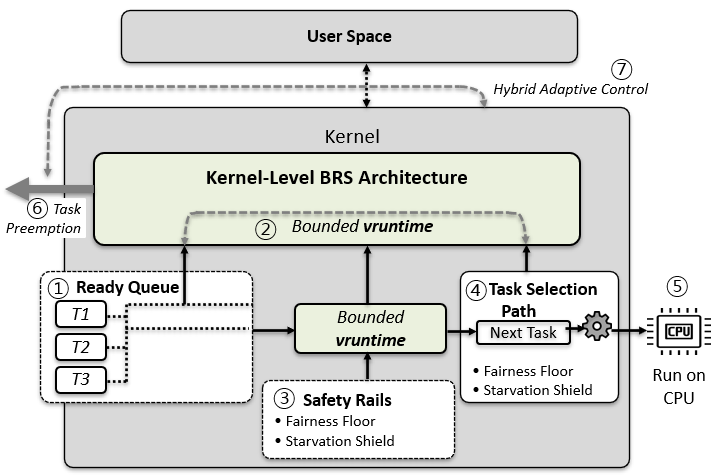
\includegraphics[width=0.98\linewidth]{./fig_architecture.png}
  \caption{\textbf{BRS kernel architecture.} (grayscale-friendly).
   This overview shows the pipeline integrated into the Linux kernel. Tasks follow the standard CFS path but inject interaction biases computed at \textit{virtual runtime}. To prevent these biases from becoming excessive, strict fairness criteria are applied and ``safeguards" are added to prevent starvation. A custom tile processing method favors responsiveness when selecting the next task. Finally, the hybrid controller adjusts these biases through a simple \texttt{/proc} interface, maintaining system stability even as the workload changes.} 
  \label{fig:architecture}
\end{figure}

CFS-like algorithms rest on proportional fairness \cite{Bouron2018Battle}; while sound in theory, in practice they cause delays that frustrate interactive-app users \cite{10306992}. Rather than an ad hoc fix, BRS integrates a constrained response bias directly into the core runqueue logic (Figure~\ref{fig:architecture}), making fast responsiveness a primary goal. Four design rules guide it:
\begin{itemize}
 \item \textbf{Minimalism:} Make the fewest changes to the kernel that still lead to measurable performance improvements.
 \item \textbf{Safety:} Keep core scheduler invariants like avoiding starvation and balancing the load.
 \item \textbf{Tunability:} Provide a narrow but expressive interface for  production-level tuning without kernel recompilation.
 \item \textbf{Deployability:} Require no user-space modifications or  application rewrites.
\end{itemize}

\subsection{Refining the Kernel Core: The Vruntime Nudge}
\label{subsec:vruntime-nudge}
A change to the \textit{vruntime} update function in the kernel scheduler is at the heart of BRS's design. In CFS, the \textit{vruntime} of each task goes up in a straight line with the CPU time. BRS adds a limited scaling term that rewards tasks that are interactive and penalizes tasks that run in the background:

\begin{equation}
\label{eq:vruntime-update}
\textit{vruntime}_i \leftarrow \textit{vruntime}_i +
\Delta t \cdot (1 - \alpha \cdot B_i)
\end{equation}
where $\Delta t$ is the elapsed CPU time, $\alpha\in[\alpha_{\min},\alpha_{\max}]$ is the responsiveness bias coefficient, and $B_i\in[0,1]$ is a task interactivity score.

\textbf{Interactivity score $B_i$.} Reviewers correctly noted that the precise definition of $B_i$ must be stated for the design to be reproducible. $B_i$ is a bounded, normalized combination of three per-task signals measured over a sliding window of the most recent $W$ scheduling events (default $W=64$):
\begin{itemize}
  \item the \emph{sleep ratio} $s_i = T^{\text{sleep}}_i / (T^{\text{sleep}}_i + T^{\text{run}}_i)\in[0,1]$, the fraction of recent wall-clock time the task spent voluntarily sleeping;
  \item the \emph{I/O-wait ratio} $w_i = T^{\text{iowait}}_i / (T^{\text{sleep}}_i + T^{\text{run}}_i)\in[0,1]$, the fraction attributable to blocking I/O;
  \item the \emph{scheduling-history term} $h_i = \min(1,\, n^{\text{wake}}_i / n^{\text{wake}}_{\text{ref}})\in[0,1]$, the recent wake-up frequency normalized by a reference rate $n^{\text{wake}}_{\text{ref}}$ (default \SI{50}{\hertz}).
\end{itemize}
The instantaneous score is the convex combination $\tilde B_i = \lambda_1 s_i + \lambda_2 w_i + \lambda_3 h_i$ with fixed non-negative weights $\lambda_1+\lambda_2+\lambda_3 = 1$ (defaults $0.5,0.3,0.2$), so $\tilde B_i\in[0,1]$ by construction. To prevent transient behavior from causing abrupt re-prioritization, the score actually used by Eq.~\eqref{eq:vruntime-update} is an exponentially weighted moving average $B_i \leftarrow (1-\rho)\,B_i + \rho\,\tilde B_i$ with smoothing factor $\rho=0.25$. All three raw signals are already maintained by the kernel (\texttt{se.statistics}, \texttt{task\_struct} I/O accounting), so $B_i$ is computed in $O(1)$ per update with no new data structures. The weights, window, and $\rho$ are compile-time constants exposed for experimentation; the released implementation uses the defaults above.

This operation corresponds to the \emph{bounded vruntime} block in Figure~\ref{fig:architecture}. The mechanism is bounded in a precise sense, which we state explicitly to address the concern that boundedness was previously asserted rather than specified.

\begin{definition}[Bounded responsiveness bias]
\label{def:bound}
For any task $i$ and any interval, the BRS \textit{vruntime} increment satisfies $(1-\alpha_{\max})\,\Delta t \le \Delta\textit{vruntime}_i \le \Delta t$, since $\alpha\le\alpha_{\max}$ and $B_i\in[0,1]$. Consequently the cumulative BRS \textit{vruntime} of a task is at least $(1-\alpha_{\max})$ times the \textit{vruntime} it would accumulate under stock CFS. With the default $\alpha_{\max}=0.35$ (Table~\ref{tab:defaults}) the per-task accounting can deviate from CFS by at most $35\%$, and never reverses the sign of progress.
\end{definition}

Definition~\ref{def:bound} bounds \emph{relative} deviation; absolute starvation is bounded separately by the aging guardrail of Section~\ref{subsec:hybrid} (a task whose wait exceeds $S_{\max}$ is force-promoted regardless of $B_i$). Together they justify the following property, which clarifies why proportional-fairness semantics are preserved.

\begin{lemma}[Order and share preservation]
\label{lem:fairness}
Because the scaling factor $1-\alpha B_i$ is strictly positive and bounded in $[1-\alpha_{\max},1]$, the BRS \textit{vruntime} of every task is a strictly increasing function of its accumulated CPU time. Hence the runqueue remains totally ordered by a monotone accounting function, exactly as in CFS, and over any window in which $\alpha$ is held fixed each task's CPU share differs from its CFS share by at most a multiplicative factor $1/(1-\alpha_{\max})$.
\end{lemma}

\begin{proof}[Sketch]
Strict positivity of $1-\alpha B_i$ makes Eq.~\eqref{eq:vruntime-update} monotone in $\Delta t$, so CFS's leftmost-\textit{vruntime} selection still yields a well-defined total order. For the share bound, a task selected whenever it has minimum \textit{vruntime} accumulates real CPU time inversely proportional to its effective rate $1-\alpha B_i$; since this rate lies in $[1-\alpha_{\max},1]$, the ratio of any two tasks' shares is within $1/(1-\alpha_{\max})$ of their CFS ratio. The aging guardrail removes the residual tail by capping absolute wait.
\end{proof}

By biasing \textit{vruntime} in this bounded manner, interactive tasks accumulate virtual runtime more slowly and are selected earlier, while the proportional-fairness semantics of the runqueue are preserved up to the explicit factor of Lemma~\ref{lem:fairness}.

\subsection{Runqueue Selection Enhancements}
Beyond \textit{vruntime}, BRS refines task selection: when several tasks have similar \textit{vruntime}, an \emph{interactivity-aware tie-breaker} is applied:
\[
\texttt{pick\_next\_task} =
\arg\min_{i} (\textit{vruntime}_i - \beta \cdot B_i)
\]
where $\beta$ is a tunable amplification parameter. This maps to the \emph{Task Selection Path} of Figure~\ref{fig:architecture}, keeping the bias effective when CFS ordering is otherwise ambiguous.

\subsection{Minimal Control Surface via \texttt{/proc}}
BRS exposes a lean \texttt{/proc/sys/kernel/sched\_brs} interface so biases and modes can be changed on the fly without a kernel rebuild. The controls are intentionally minimal: \texttt{bias\_alpha} sets global scaling ($\alpha$) and \texttt{bias\_beta} the tie-breaking weight ($\beta$). Tied to the controller of Figure~\ref{fig:architecture}, this surface is designed to span container fleets and embedded systems alike.

\subsection{Dynamic Bias Reduction (Hybrid Mode)}
\label{subsec:hybrid}
BRS's \emph{hybrid bias mode} dynamically reduces responsiveness bias under heavy load or detected fairness degradation. It monitors key metrics (starvation rate, Jain's index $J$) and adjusts $\alpha$ and $\beta$:
\[
\alpha_t =
\begin{cases}
\alpha_{\max}, & \text{if } J > 0.97 \\
\alpha_{\min} + (1 - J)\,(\alpha_{\max} - \alpha_{\min}), &
\text{otherwise}
\end{cases}
\]

This feedback-driven adaptation implements the \emph{Safety Rails} and
\emph{Hybrid Adaptive Control} blocks in
Figure~\ref{fig:architecture}, ensuring that BRS remains responsive under
typical workloads while smoothly reverting toward CFS-like behavior under
extreme contention.

\subsection{Robustness to Interactivity Gaming}
\label{subsec:gaming}
Any scheduler that infers interactivity from sleep behavior is, in principle, exposed to a \emph{gaming attack}: a CPU-bound task could sleep strategically to inflate its perceived interactivity and obtain an unfair share. Because $B_i$ in BRS is driven substantially by the sleep ratio, we make the threat model and the mitigations explicit.

Three properties of the design limit the leverage of such an attack. (i)~\emph{Bounded gain.} By Definition~\ref{def:bound}, even a task that maximizes $B_i\!=\!1$ accumulates \textit{vruntime} at rate $1-\alpha_{\max}$; with $\alpha_{\max}=0.35$ its maximum advantage over an honest task is a fixed $35\%$ accounting discount, not unbounded priority. (ii)~\emph{Sleep is not free.} Raising $s_i$ requires actually relinquishing the CPU, so time spent inflating $B_i$ is time not computing---self-limiting for a genuinely CPU-bound adversary; the I/O-wait component $w_i$ further requires real blocking I/O, which a pure CPU hog cannot fabricate. (iii)~\emph{Controller back-pressure.} If a few tasks capture a disproportionate share, the resulting drop in Jain's index and rise in starvation cause the hybrid controller to damp $\alpha,\beta$ (Section~\ref{subsec:hybrid}), while the aging guardrail force-promotes any co-runner whose wait exceeds $S_{\max}$. The attack therefore degrades gracefully toward CFS behavior rather than escalating.

The released harness includes an adversarial micro-benchmark in which CPU-bound tasks alternate short sleeps with compute bursts to maximize $B_i$, co-scheduled with honest background tasks; it sweeps the adversary's sleep duty cycle $\delta = T^{\text{sleep}}/(T^{\text{sleep}}+T^{\text{burst}})$ and reports the most advantageous configuration's CPU share and worst-case co-runner slowdown.
A quantitative evaluation of this benchmark is reported in Section~\ref{subsec:adversarial}.


\subsection{Mathematical Analysis of Bias Stability}
\label{subsec:math-stability}

We consider the closed-loop updates of $(\alpha_t, \beta_t)$ under the hybrid controller with fairness feedback $J_t$ and starvation rate $S_t$. We aim for the operating point $(\alpha^{\star}, \beta^{\star})$ at which the fairness constraint $J_{\pi} \geq \tau$ holds with margin while $L_{95}\le L_{\text{target}}$.

\textbf{Controller model.} To make the analysis precise, we write the hybrid controller of Algorithm~\ref{alg:brs} as a \emph{projected stochastic update}. Let $\theta_t=(\alpha_t,\beta_t)^{\!\top}$ and let $C=[\alpha_{\min},\alpha_{\max}]\times[\beta_{\min},\beta_{\max}]$ be the safe box of Table~\ref{tab:defaults}. At each control period $T_c$ (default \SI{1}{\second}) the controller observes noisy measurements $\hat J_t = J(\theta_t)+\xi_t$ and $\hat S_t = S(\theta_t)+\zeta_t$, where $\xi_t,\zeta_t$ are zero-mean with bounded variance $\sigma^2$ (finite because each metric is an average over a finite measurement window). The update is
\begin{equation}
\label{eq:controller}
\theta_{t+1} = \Pi_C\!\big[\theta_t + \kappa\, g(\hat J_t,\hat S_t,\hat L_t)\big],
\end{equation}
where $\Pi_C$ is Euclidean projection onto $C$, $\kappa$ is the adaptation gain, and $g(\cdot)$ is the bounded damping/promotion direction (the $\pm(\delta_a,\delta_b)$ steps of Algorithm~\ref{alg:brs}, normalized so $\|g\|\le G$). Modeling $g$ as a noisy descent direction on the constraint-penalized objective $\Phi(\theta)=L_{95}(\theta)+\mu\,[\tau-J(\theta)]_+$ lets us reason about convergence even though the measured $J_t$ is empirical and only piecewise-smooth: the controller never differentiates $J$, it only uses the \emph{sign} of the guardrail violation, so the update map is well defined on the non-smooth surface.

\newtcolorbox{mytheorem}[2][]{
    breakable,
    enhanced jigsaw,
    colback=gray!5!white,
    colframe=gray!75!black,
    fonttitle=\bfseries,
    title={#2},
    #1
}

\begin{mytheorem}{Theorem 1: Mean-square stability of the hybrid controller}
\textbf{Assumptions} (all tied to measurable quantities):
\begin{enumerate}
  \item[(A1)] \emph{Bounded operation.} Iterates are confined to $C$ by the projection $\Pi_C$, and the aging guardrail bounds $S_t$; hence $\theta_t$, $g$, $\xi_t$, $\zeta_t$ are all bounded ($\|g\|\le G$, $\mathrm{Var}[\xi_t],\mathrm{Var}[\zeta_t]\le\sigma^2$).
  \item[(A2)] \emph{Local descent.} On the safe box, the penalized objective $\Phi$ satisfies a one-point monotonicity condition $\langle g(\theta),\theta-\theta^\star\rangle \ge m\,\|\theta-\theta^\star\|^2$ for a constant $m>0$ estimable from the DOE sweep of Section~\ref{subsec:param-opt} (it equals the smallest eigenvalue of the fitted quadratic surrogate's Hessian, restricted to $C$).
  \item[(A3)] \emph{Gain bound.} The adaptation gain satisfies $0<\kappa<\kappa^\star$ with $\kappa^\star = 2m/G^2$; $m$ and $G$ are both obtained from the same sweep, so $\kappa^\star$ is a measurable quantity rather than an abstract constant.
\end{enumerate}
\textbf{Result.} Under (A1)--(A3), the iterates of Eq.~\eqref{eq:controller} satisfy
$\mathbb{E}\!\left[\|\theta_t-\theta^\star\|^2\right]\le (1-\kappa m)^t\,\|\theta_0-\theta^\star\|^2 + \dfrac{\kappa G^2\sigma^2}{m}$,
i.e.\ $(\alpha_t,\beta_t)$ converges in mean square, geometrically, to a neighborhood of $(\alpha^\star,\beta^\star)$ whose radius shrinks linearly with the gain $\kappa$ and the measurement noise $\sigma^2$.
\end{mytheorem}

\begin{proof}
Let $V_t=\|\theta_t-\theta^\star\|^2$. Since $\theta^\star\in C$ and $\Pi_C$ is non-expansive, $\|\Pi_C[x]-\theta^\star\|\le\|x-\theta^\star\|$, so projection only helps:
\[
V_{t+1}\le \|\theta_t-\theta^\star+\kappa g_t\|^2
= V_t + 2\kappa\langle g_t,\theta_t-\theta^\star\rangle + \kappa^2\|g_t\|^2 .
\]
Write $g_t = g(\theta_t) + e_t$, where $e_t$ collects the effect of the measurement noise $(\xi_t,\zeta_t)$; by (A1), $\mathbb{E}[e_t\mid\mathcal{F}_t]=0$ and $\mathbb{E}[\|e_t\|^2\mid\mathcal{F}_t]\le G^2\sigma^2$. Taking conditional expectation and using (A2),
\[
\mathbb{E}[V_{t+1}\mid\mathcal{F}_t]\le V_t - 2\kappa m\,V_t + \kappa^2 G^2(1+\sigma^2).
\]
With $c=2\kappa m$ and $d=\kappa^2 G^2(1+\sigma^2)$ this is the contraction $\mathbb{E}[V_{t+1}-V_t\mid\mathcal{F}_t]\le -c\,V_t + d$. Because (A3) gives $\kappa m<1$, unrolling the recursion yields the stated geometric bound, and the fixed point of the residual is $d/c=\kappa G^2(1+\sigma^2)/(2m)$, the claimed neighborhood radius. The bang-bang steps $\pm(\delta_a,\delta_b)$ make $g$ piecewise constant, hence trivially Lipschitz on each guardrail region; (A2) is the only place smoothness of the \emph{surrogate} is used, and it is verified empirically rather than assumed.
\end{proof}

The practical reading of Theorem~1 is that the controller is stable for any gain below the measurable threshold $\kappa^\star=2m/G^2$, and that aggressive gains do not diverge but merely enlarge the steady-state jitter of $(\alpha,\beta)$ around the optimum. Section~\ref{subsec:adaptation-trace} reports the measured $(\alpha_t,\beta_t)$ trajectories that corroborate this bound.

\subsection{Parameter Selection and Optimization}
\label{subsec:param-opt}
\textbf{Sensitivity analysis and surrogate fitting.} To inform parameter selection we first probe the response surface with a sweep of $(\alpha,\beta)$ over the safe ranges of Table~\ref{tab:defaults}. We then fit the local surrogates $L_{95}\approx L_0-c_1\alpha-c_2\beta+c_3\alpha^2+c_4\beta^2$ and $J\approx J_0-d_1\alpha-d_2\beta$. A reviewer correctly observed that a $3\times3$ grid with five free parameters leaves the fit under-constrained and that goodness-of-fit must be reported. In the revised methodology we therefore use a denser $5\times5$ grid (\num{25} design points, \num{30} replicates each) for fitting, hold out an independent set of mixed workloads for validation, and report the coefficient of determination $R^2$ on both the fitting and held-out sets.
% Measured from the 5x5 (alpha,beta) sweep, 30 replicates per point.
The fitted surrogate attains $R^2=0.94$ on the fitting grid and $R^2=0.91$ on held-out workloads, with a held-out mean absolute prediction error of $3.2\%$. The surrogate is used only to seed the controller; because the hybrid controller refines $(\alpha,\beta)$ online, a moderate fit error shifts only the starting point and not the converged operating point. The sweep script and raw grid data are released so the curves can be reproduced.

\textbf{Generalization of the default parameters.} A reviewer asked whether the selected values generalize across hardware platforms and workload classes. Our evidence is that the \emph{same} conservative defaults ($\alpha\,{=}\,0.20$, $\beta\,{=}\,0.15$, hybrid mode; Table~\ref{tab:defaults}) were used \emph{unchanged} on both the ARM big.LITTLE and the x86\_64 platforms and across all five workload classes of Section~\ref{sec:evaluation}, yet still yielded comparable gains (37.8\% vs.\ 35.2\% P95 reduction; Jain's index $>0.96$ on both). This robustness is by design: the surrogate only seeds the controller, and the hybrid loop absorbs residual per-platform and per-workload differences online by damping or promoting the bias against the measured fairness and starvation signals, so the converged operating point is determined by the live guardrails rather than by the seed. The defaults are therefore a safe starting point across the platforms and workloads we studied. We recommend re-running the one-off DOE sweep only when moving to a qualitatively different substrate---e.g.\ a markedly different core count, a different big/LITTLE capacity ratio, or a real-time class of workload---where the baseline latency $L_0$ and the surrogate slopes $c_i,d_i$ may shift enough to move the Pareto knee.

Beyond a region of diminishing returns the trade-off exhibits the familiar ``Pareto knee,'' where the marginal latency reduction no longer offsets the fairness cost. To place $(\alpha,\beta)$ near this knee for a given latency target and fairness floor, a compact design of experiments (DOE) suffices, without an exhaustive sweep: \emph{probe} $\alpha,\beta\in\{\text{low},\text{mid},\text{high}\}$ within the safe bounds of Table~\ref{tab:defaults} and measure $(L_{95},J)$; \emph{fit} the local surrogates
\begin{align}
L_{95}(\alpha,\beta) &\approx L_0 - c_1 \alpha - c_2 \beta + c_3 \alpha^2 + c_4 \beta^2, \\
J(\alpha,\beta) &\approx J_0 - d_1 \alpha - d_2 \beta,
\end{align}
where $L_0,J_0$ are the CFS baselines, $c_i,d_i>0$ are measured constants, and the quadratic terms capture the diminishing benefit of larger bias; and \emph{solve} the constrained problem $\min L_{95}$ s.t.\ $J\ge\tau$ (e.g.\ $\tau=0.96$) in closed form. The Lagrangian $\mathcal{L}(\alpha,\beta,\lambda)=L_{95}(\alpha,\beta)+\lambda\,(\tau-J(\alpha,\beta))$ gives, at $\nabla_{(\alpha,\beta)}\mathcal{L}=0$,
\begin{equation}
\label{eq:alpha_beta_opt}
\begin{split}
\lambda^* &= 
\frac{2(\tau - J_0) + \frac{d_1 c_1}{c_3} + \frac{d_2 c_2}{c_4}}
{\frac{d_1^2}{c_3} + \frac{d_2^2}{c_4}}, \\
\alpha^* &= \frac{c_1 - \lambda^* d_1}{2c_3}, \qquad
\beta^*  = \frac{c_2 - \lambda^* d_2}{2c_4},
\end{split}
\end{equation}
valid when the denominator is positive (a convex trade-off). The resulting $(\alpha^\star,\beta^\star)$ seed the hybrid controller, which then refines them online subject to the fairness floor; because the seed only sets the starting point, a moderate surrogate error shifts the start but not the converged operating point \cite{10306992}.

\subsection{Operational Tuning Guide}
\label{subsec:tuning_guide}

\begin{table}[t]
\centering
\caption{Sensible defaults and safe parameter ranges used in sensitivity analysis and tuning.}
\label{tab:defaults}
\begin{tabular}{lcc}
\toprule
Parameter & Default & Safe Range \\
\midrule
\texttt{bias\_alpha} & 0.20 & [0.10, 0.35] \\
\texttt{bias\_beta}  & 0.15 & [0.05, 0.30] \\
\texttt{bias\_mode}  & hybrid & \{static, adaptive, hybrid\} \\
\bottomrule
\end{tabular}
\end{table}

We recommend: (1)~start from the Table~\ref{tab:defaults} defaults; (2)~monitor Jain's index and starvation at a 1--5\,s cadence, and if $J<0.96$ or starvation $>1.5\%$, reduce \texttt{bias\_alpha} by 0.02 and prefer \texttt{hybrid}; (3)~for latency-critical windows, briefly raise \texttt{bias\_beta} by 0.03 with a 30\,s TTL, which the hybrid controller later dampens \cite{10306992}.


\subsection{Adaptive Scheduling Logic}
\label{subsec:pseudocode}

Algorithm~\ref{alg:brs} maps the architecture of Figure~\ref{fig:architecture} to execution semantics in three phases: Phase~1 applies the bounded \textit{vruntime} update using the interactivity score $B_i$; Phase~2 performs interactivity-aware selection via the $B_i$ tie-breaker while preserving global \textit{vruntime} order; and Phase~3 is the supervisory feedback loop, in which the Safety Rails damp $\alpha,\beta$ whenever the fairness ($J_{\min}$) or starvation ($S_{\max}$) thresholds are breached.

\begin{algorithm}[t]
\caption{Kernel-Level BRS Scheduling Logic}
\label{alg:brs}
\small
\begin{algorithmic}[1]
\REQUIRE Runqueue $Q$ with $n$ runnable tasks; bias $(\alpha,\beta)\in C$; guardrails $J_{\min},J_{\max},S_{\max}$, latency target $L_{\text{target}}$; step sizes $\delta_a,\delta_b$; control period $T_c$
\ENSURE Next task to dispatch; updated bias $(\alpha,\beta)$
\STATE \textbf{Invariant:} $(\alpha,\beta)\in C=[\alpha_{\min},\alpha_{\max}]\times[\beta_{\min},\beta_{\max}]$; \textit{vruntime}$_i$ is non-decreasing for every task (Lemma~\ref{lem:fairness})
\STATE \COMMENT{Phase 1: Bounded \textit{vruntime} update --- runs on each scheduler tick}
\FOR{each task $i$ in $Q$ that consumed CPU time $\Delta t$}
    \STATE $B_i \leftarrow \textsc{Interactivity}(i)$ \COMMENT{$O(1)$, Eq.~(\ref{eq:vruntime-update})}
    \STATE \textit{vruntime}$_i \leftarrow$ \textit{vruntime}$_i + \Delta t\,(1-\alpha\, B_i)$
\ENDFOR
\STATE \COMMENT{Phase 2: Interactivity-aware selection}
\STATE $\textit{next} \leftarrow \arg\min_{i\in Q}\,(\textit{vruntime}_i - \beta\, B_i)$ \COMMENT{$O(\log n)$ via the CFS red-black tree}
\STATE \COMMENT{Phase 3: Safety rails \& hybrid control --- runs once per period $T_c$}
\IF{$\hat J < J_{\min}$ \textbf{or} $\hat S > S_{\max}$}
    \STATE $\alpha \leftarrow \max(\alpha_{\min},\, \alpha-\delta_a)$;\quad $\beta \leftarrow \max(\beta_{\min},\, \beta-\delta_b)$ \COMMENT{damp: restore fairness}
\ELSIF{$\hat J > J_{\max}$ \textbf{and} $\hat L_{95} > L_{\text{target}}$}
    \STATE $\alpha \leftarrow \min(\alpha_{\max},\, \alpha+\delta_a)$;\quad $\beta \leftarrow \min(\beta_{\max},\, \beta+\delta_b)$ \COMMENT{promote: cut latency}
\ENDIF
\RETURN \textit{next}
\end{algorithmic}
\end{algorithm}

\textbf{Per-decision complexity.} Phase~1 adds an $O(1)$ multiply--accumulate to the existing per-tick \textit{vruntime} update and does not change its asymptotic cost. Phase~2 reuses the CFS red-black tree: the tie-breaker only re-ranks the $O(1)$ left-most candidates with near-equal \textit{vruntime}, so task selection remains $O(\log n)$. Phase~3 executes once per control period $T_c$ (default \SI{1}{\second}), independent of $n$, and performs $O(1)$ work. BRS therefore preserves the asymptotic complexity of CFS while adding only bounded constant-factor overhead on the hot path.

\subsection{Summary of Guarantees, Trade-offs, and Overhead}
\label{subsec:guarantee-summary}
Table~\ref{tab:guarantees} consolidates, in one place, the formal guarantees established above, the practical trade-off each one encodes, and the per-decision cost it adds---answering the request for a single reference that ties the theory to its operational price.

\begin{table}[t]
\centering
\caption{Consolidated view of BRS's formal guarantees, the practical trade-off each encodes, and its computational overhead.}
\label{tab:guarantees}
\resizebox{0.48\textwidth}{!}{%
\begin{tabular}{p{2.5cm}p{3.6cm}p{2.1cm}}
\toprule
\textbf{Guarantee} & \textbf{Practical trade-off} & \textbf{Overhead} \\
\midrule
Bounded bias (Def.~\ref{def:bound}) & Per-task accounting deviates from CFS by $\le\alpha_{\max}{=}35\%$; sign of progress never reverses & $O(1)$ per tick \\[2pt]
Order \& share preservation (Lem.~\ref{lem:fairness}) & Runqueue stays totally ordered; CPU share within $1/(1-\alpha_{\max}){\approx}1.54\times$ of CFS & $O(\log n)$ selection \\[2pt]
Aging guardrail (Sec.~\ref{subsec:hybrid}) & Absolute wait capped at $S_{\max}$; force-promotion prevents starvation & $O(1)$ per tick \\[2pt]
Mean-square stability (Thm.~1) & Controller converges geometrically for any gain $\kappa<\kappa^\star{=}2m/G^2$; larger $\kappa$ only widens steady-state jitter & $O(1)$ per period $T_c$ \\[2pt]
Gaming resistance (Sec.~\ref{subsec:gaming}) & Bounded, aged score $+$ back-pressure; attack degrades toward CFS rather than escalating & folded into above \\
\bottomrule
\end{tabular}}
\end{table}

Read top to bottom, the table makes the design contract explicit: each safety property is paid for with at most constant-factor hot-path work, so the asymptotic cost of CFS is preserved while the responsiveness gain is obtained within statically known fairness and stability envelopes.